\documentclass[%
    %handout
]{beamer}
\usepackage{graphicx} % For including single page pdfs
\usepackage{bm}       % bold math
\usepackage{pgffor}   % for loop
\usepackage{tikz}
\usepackage{multimedia}
\usepackage{layouts}
%\usepackage[colorlinks=false,allbordercolors={0 0 0},pdfborderstyle={/S/U/W 1}]{hyperref}

\usepackage{cambridge_lecture}
\hypersetup{colorlinks=false,pdfborderstyle={/S/U/W 1}}

% todo 
% - Ligo actual data
% -define IMRPhenom, EOBNR


\newcommand{\lik}{\mathcal{L}}
\newcommand{\posterior}{\mathcal{P}}
\newcommand{\prior}{\pi}
\newcommand{\ev}{\mathcal{Z}}

\newcommand{\prob}{\mathrm{P}}

\newcommand{\PR}{\mathcal{P}_\mathcal{R}}
\newcommand{\Pknotj}[1]{\mathcal{P}_{#1}}
\newcommand{\Nknots}{N_\text{knots}}
\newcommand{\nlive}{n_\text{live}}

\newcommand{\movablecross}[1]{%
  \draw[->](#1) -- ++(0:\croslen);
  \draw[->](#1) -- ++(90:\croslen);
  \draw[->](#1) -- ++(180:\croslen);
  \draw[->](#1) -- ++(270:\croslen);
  \fill[red!70!black] (#1) circle (2pt);
}

\newcommand{\movablevert}[1]{%
  \draw[->](#1) -- ++(90:\croslen);
  \draw[->](#1) -- ++(270:\croslen);
  \fill[red!70!black] (#1) circle (2pt);
}

%Nested Sampling: an efficient and robust Bayesian inference tool for
%astrophysics and cosmology
%
%Nested sampling is an alternative MCMC technique for integrating and exploring
%probability distributions. It has become widely adopted in the field of
%cosmology as the de-facto tool for computing Bayesian evidences and sampling
%challenging a-priori unknown parameter spaces.
%
%In this talk, I will give an introduction to the principles of Bayesian model
%comparison and parameter estimation, an explanation of the theory of nested
%sampling, a survey of the current state-of-the art (MultiNest, PolyChord,
%DNest and Dynesty) and the future of the field. Throughout I will illustrate
%with examples of it's application in cosmology and astrophysics, ranging from
%inflationary physics to exoplanets.





\setbeamertemplate{navigation symbols}{} % Turn off that bottom bar


\title{Bayesian statistics}
\subtitle{Third ASTERICS-OBELICS Workshop}
\author[Handley] % (optional, for multiple authors)
{Will Handley\\ \small{wh260@cam.ac.uk}}
\institute[University of Cambridge] % (optional)
{%
Kavli Institute for Cosmology\\
Cavendish Laboratory (Astrophysics Group) \\
University of Cambridge
}
\date{October 24, 2018}

\usepackage{calculator}

\newcommand{\cols}[3][0.5]{%
    \SUBTRACT{1.}{#1}{\wdthb}
    \begin{columns}
        \begin{column}{#1\textwidth}
            #2
        \end{column}
        \begin{column}{\wdthb\textwidth}
            #3
        \end{column}
    \end{columns}
}

\newcommand{\figname}{}
\newenvironment{figright}[2][0.5]{%
    \renewcommand{\figname}{#2}
    \SUBTRACT{1.}{#1}{\wdthb}
    \begin{columns}
        \begin{column}{#1\textwidth}
        }{%
        \end{column}
        \begin{column}{\wdthb\textwidth}
            \includegraphics[width=\textwidth]{\figname}
        \end{column}
    \end{columns}
}

\newcommand{\dfigname}{}
\newenvironment{dfigright}[3][0.5]{%
    \renewcommand{\figname}{#2}
    \renewcommand{\dfigname}{#3}
    \SUBTRACT{1.}{#1}{\wdthb}
    \begin{columns}
        \begin{column}{#1\textwidth}
        }{%
        \end{column}
        \begin{column}{\wdthb\textwidth}
            \includegraphics[width=\textwidth]{\figname}
            \includegraphics[width=\textwidth]{\dfigname}
        \end{column}
    \end{columns}
}



\newenvironment{figleft}[2][0.5]{%
    \SUBTRACT{1.}{#1}{\wdthb}
    \begin{columns}
        \begin{column}{#1\textwidth}
            \includegraphics[width=\textwidth]{#2}
        \end{column}
        \begin{column}{\wdthb\textwidth}
        }{%
        \end{column}
    \end{columns}
}

\newenvironment{dfigleft}[3][0.5]{%
    \SUBTRACT{1.}{#1}{\wdthb}
    \begin{columns}
        \begin{column}{#1\textwidth}
            \includegraphics[width=\textwidth]{#2}
            \includegraphics[width=\textwidth]{#3}
        \end{column}
        \begin{column}{\wdthb\textwidth}
        }{%
        \end{column}
    \end{columns}
}


\newcounter{numimages}

\newenvironment{multifig}[1]{%
    \begin{frame}
        \pdfximage{#1}%
        \setcounter{numimages}{\the\pdflastximagepages}
        \addtocounter{numimages}{-1}

        \begin{tikzpicture}[remember picture, overlay]
            \foreach \pagenum in {1,...,\thenumimages} {%
                \node<handout:0|beamer:\pagenum>[anchor=center] at (current page.center) {
                \includegraphics[width=\textwidth,page=\pagenum]{#1}}; 
            }
            \addtocounter{numimages}{1}
            \node<handout:1|beamer:\thenumimages>[anchor=center] at (current page.center) {
            \includegraphics[width=\textwidth,page=\thenumimages]{#1}}; 
        \end{tikzpicture}
    }{%
    \end{frame}
}



\begin{document}

\begin{frame}
  \titlepage
\end{frame}

\begin{frame}
  \frametitle{Inference in cosmology: parameter estimation}
    \begin{figright}[0.4]{./figures/age_size.pdf}
        \begin{itemize}
            \item Cosmologists infer universe parameters from data
            \item Bayesian framework: Use probability distributions to quantify errors
            \item Inferences depend on models ($\Lambda$CDM)
            \item \href{https://arxiv.org/abs/1807.06209}{arXiv:1807.06209}
        \end{itemize}
    \end{figright}
\end{frame}

\begin{frame}
  \frametitle{Inference in cosmology: model comparison}
    \begin{figright}[0.4]{./figures/age_size_curved.pdf}
        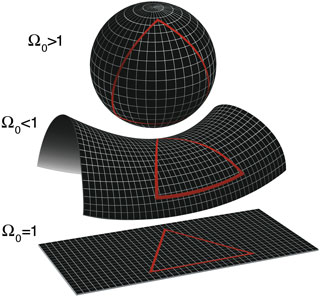
\includegraphics[width=\textwidth]{./figures/shape-of-the-universe}
        \begin{itemize}
            \item Green model includes curvature (c$\Lambda$CDM)
            \item Age and size now correlated
            \item Measurement less precise
            \item Flat is better with 2:1 odds against curvature
        \end{itemize}
    \end{figright}
\end{frame}

\section{Fitting a line to data}
\begin{frame}
    \frametitle{Motivating example: Fitting a line to data}
    \begin{figright}[0.4]{./figures/data_points.pdf}
        \begin{itemize}
            \item We have noisy data $D$
            \item We wish to fit a model $M$
            \item Functional form $y=f_M(x;\theta)$
            \item For example:
                \begin{align}
                     f_\text{linear}(x;\theta)&=a x + b       \nonumber\\
                     f_\text{quadratic}(x;\theta)&=a x^2 + b  \nonumber
                \end{align}
            \item Model parameters $\theta= (a,b)$
        \end{itemize}
    \end{figright}
\end{frame}

\begin{frame}
    \frametitle{$\chi^2$ best-fit}
    \framesubtitle{Fitting lines to data}
    \begin{figright}[0.4]{./figures/data_diff.pdf}
        \begin{itemize}
            \item For each parameter set $\theta$:
                \[
                    \chi^2(\theta) = \sum_i \left|y_i - f(x_i;\theta)\right|^2
                \]
            \item Minimise $\chi^2$ wrt $\theta$
        \end{itemize}
    \end{figright}
\end{frame}

\begin{frame}
    \frametitle{$\chi^2$ with non-uniform data errors}
    \framesubtitle{Fitting lines to data}
    \begin{figright}[0.4]{./figures/data.pdf}
        \begin{itemize}
            \item If data have non-uniform errors:
                \[
                    \chi^2(\theta) = \sum_i \frac{\left|y_i - f(x_i;\theta)\right|^2}{\sigma_i^2}
                \]
        \end{itemize}
    \end{figright}
\end{frame}

\begin{frame}
    \frametitle{Problems with $\chi^2$}
    \framesubtitle{Fitting lines to data}
    \begin{figright}[0.4]{./figures/data_diff_2.pdf}
        \begin{itemize}
            \item Why square the errors? -- could take absolute:
                \[
                    \psi^2(\theta) = \sum_i \frac{\left|y_i - f(x_i;\theta)\right|}{\sigma_i}
                \]
            \item How do we differentiate between models, e.g. quadratic vs curved
        \end{itemize}
    \end{figright}
\end{frame}

\begin{frame}
    \frametitle{Probability distributions}
    \framesubtitle{Fitting lines to data}
    \begin{figright}[0.6]{./figures/data_diff_1.pdf}
        \begin{itemize}
            \item The probability of observing a datum:
                \[
                    P(y_i | \theta,M) = \frac{1}{\sqrt{2\pi}\sigma_i}\exp\left({-\frac{|y_i-f(x_i;\theta)|^2}{2\sigma_i^2}}\right)
                \]
            \item The probability of observing the data:
                \begin{align}
                    P(D | \theta,M) &= \prod_i \frac{1}{\sqrt{2\pi}\sigma_i}\exp\left({-\frac{|y_i-f(x_i;\theta)|^2}{2\sigma_i^2}}\right) \nonumber\\
                    &=  \frac{1}{\prod_i\sqrt{2\pi}\sigma_i}\exp\sum_i{-\frac{|y_i-f(x_i;\theta)|^2}{2\sigma_i^2}} \nonumber\\
                    &\propto e^{-\chi^2(\theta)/2}
                    \nonumber
                \end{align}
        \end{itemize}
    \end{figright}
\end{frame}



\begin{frame}
    \frametitle{Maximum likelihood}
    \framesubtitle{Fitting lines to data}
    \begin{figleft}[0.6]{./figures/data_diff.pdf}
        \begin{itemize}
            \item Minimising $\chi^2(\theta)$  is equivalent to maximising $P(D|\theta,M) \propto e^{-\chi^2(\theta)/2}$
            \item $P(D|\theta,M)$ is called the Likelihood $L=L(\theta)$ of the parameters $\theta$
            \item ``Least squares'' $\equiv$ ``maximum likelihood'' \\(if data are gaussian).
            \item \href{https://arxiv.org/abs/1809.04598}{arXiv:1809.04598}
        \end{itemize}
    \end{figleft}
\end{frame}

\begin{frame}
    \frametitle{Bayesian inference}
    \begin{itemize}
        \item Likelihood $L=P(D|\theta,M)$ is undeniably correct.
        \item Frequentists construct inference techniques purely from this function.
        \item The trend is cosmology is to work with a Bayesian approach.
        \item What we want are things like $P(\theta|D,M)$ and $P(M|D)$.
        \item To invert the conditionals, we need Bayes theorem:
            \begin{align}
                P(\theta|D,M) &= \frac{P(D|\theta,M) P(\theta|M)}{P(D|M)} \nonumber\\
                P(M|D) &= \frac{P(D|M) P(M)}{P(D)} \nonumber
            \end{align}
    \end{itemize}
\end{frame}

\begin{frame}
    \frametitle{Terminology}
    \framesubtitle{Bayesian inference}
    \begin{align}
        P(\theta|D,M) &= \frac{P(D|\theta,M) P(\theta|M)}{P(D|M)} \nonumber\\
        \text{Posterior} &= \frac{\text{Likelihood}\times\text{Prior}}{\text{Evidence}} \nonumber
    \end{align}
    \begin{align}
        P(M|D) &= \frac{P(D|M) P(M)}{P(D)} \nonumber\\
        \text{Model probability} &= \frac{\text{Evidence}\times\text{Model Prior}}{\text{Normalisation}} \nonumber
    \end{align}
\end{frame}

\begin{frame}
    \frametitle{The prior}
    \framesubtitle{Example: Biased coins}
    \begin{itemize}
        \item Need to define the \textbf{Prior} $P(\theta)$ --- probability of the bias, given no data
        \item Represents our knowledge of parameters before the data -- subjective
        \item Frequentists view this as a flaw in Bayesian inference. 
        \item Bayesians view this as an advantage
        \item Fundamental rule of Inference:\pause\\
            \vfill
            \begin{center}
                \Large You cannot extract information from data\\ without making assumptions 
            \end{center}
            \vfill
        \item All Bayesians do is make them explicit
        \item Any method that claims it is ``objective'' is simply hiding them
    \end{itemize}
\end{frame}

\begin{frame}
    \frametitle{Parameter estimation}
    \framesubtitle{Bayesian inference}
    \begin{figright}[0.3]{./figures/parameters.pdf}
        \begin{itemize}
            \item We may use $P(\theta|D,M)$ to inspect whether a model looks reasonable
        \end{itemize}
        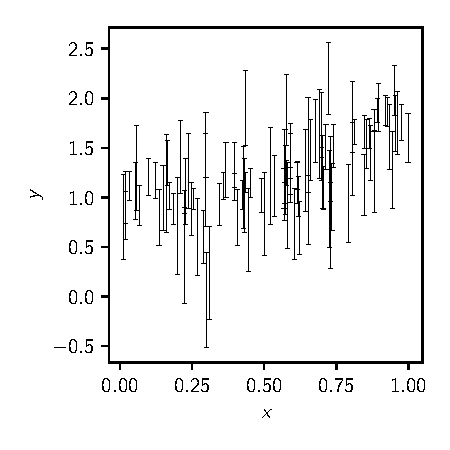
\includegraphics[width=\textwidth]{./figures/data.pdf}
    \end{figright}
\end{frame}

\begin{frame}
    \frametitle{Predictive posterior}
    \begin{figright}[0.25]{./figures/fgivenx.pdf}
        More useful to plot:
        \begin{align}
        &P(y|x) = \nonumber\\
        &\int P(y|x,\theta) P(\theta) d\theta \nonumber
        \end{align}
        (all conditioned on $D,M$)
    \end{figright}
\end{frame}

\begin{frame}
    \frametitle{Model comparison}
    \framesubtitle{Bayesian inference}
    \begin{figright}[0.33]{./figures/evidences_lin.pdf}
        \begin{itemize}
            \item We may use the Bayesian evidence $Z$ to determine whether a model is reasonable.
            \item $Z = P(D|M) = \int P(D|M,\theta)P(\theta|M)d\theta$
            \item The evidence quantifies Occam's razor, penalising over-fitted models with too many parameters.
            \item Normally assume uniform model priors $Z \propto P(M|D)P(M)$.
        \end{itemize}
    \end{figright}
\end{frame}

\begin{frame}
    \frametitle{Line fitting (context)}
    \begin{figright}[0.5]{./figures/supernovae.pdf}
        \begin{itemize}
            \item Whilst this model seems a little trite\ldots
            \item\ldots determining polynomial indices \\$\equiv$ determining cosmological material content:
        \end{itemize}
    \end{figright}
        \[
            {\left( \frac{H}{H_0} \right)}^2 = 
            \Omega_\text{r} {\left( \frac{a_0}{a} \right)}^4+
            \Omega_\text{m} {\left( \frac{a_0}{a} \right)}^3+
            \Omega_k {\left( \frac{a_0}{a} \right)}^2+
            \Omega_\Lambda
            \]
\end{frame}



\begin{frame}
    \frametitle{Quantifying error with Probability}

    \begin{figright}[0.5]{./figures/ligo_m1_m2.pdf}
        \begin{itemize}
            \item As scientists, we are used to seeing error bars on results.
            \item Masses of LIGO GW150914 binary merger: 
            \[m_1 = 39.4^{+5.5}_{-4.9}\:M_\odot\]
            \[ m_2 = 30.9^{+4.8}_{-4.4}\:M_\odot \]
            \item These are called {\em credible intervals}, state that we are e.g.\ $90\%$ confident of the value lying in this range.
            \item More importantly, these are {\em summary statistics}.
        \end{itemize}
    \end{figright}
\end{frame}


\begin{frame}
    \frametitle{Sampling}
    \framesubtitle{How to describe a high-dimensional posterior}

    \begin{figright}[0.4]{./figures/age_size_curved.pdf}
		\begin{itemize}
          \item In high dimensions, posterior $\posterior$ occupies a vanishingly small region of the prior $\prior$.
          \item Gridding is doomed to failure for $D\gtrsim4$.
          \item {\em Sampling\/} the posterior is an excellent compression scheme.
          \item Name of the game: \\ Constructing algorithms to generate samples with a minimum number of likelihood calls
		\end{itemize}
	\end{figright}
\end{frame}

\begin{frame}
    \frametitle{Sampling}
    \framesubtitle{How to describe a high-dimensional posterior}

    \begin{figright}[0.4]{./figures/age_size_curved_samples.pdf}
		\begin{itemize}
          \item In high dimensions, posterior $\posterior$ occupies a vanishingly small region of the prior $\prior$.
          \item Gridding is doomed to failure for $D\gtrsim4$.
          \item {\em Sampling\/} the posterior is an excellent compression scheme.
          \item Name of the game: \\ Constructing algorithms to generate samples with a minimum number of likelihood calls
		\end{itemize}
	\end{figright}
\end{frame}



%\section{Metropolis Hastings}
%
%
\begin{frame}
    \frametitle{Sampling algorithms: Metropolis Hastings} 
    \begin{itemize}

        \item Turn the $N$-dimensional problem into a one-dimensional one.
            \begin{enumerate}
                \item Propose random step to new point $x_{i} \to x_{i+1}$
                \item If uphill [$P(x_{i+1})>P(x_i)$], make step\ldots
                \item \ldots otherwise make step with probability $\propto P(x_{i+1})/P(x_i)$. 
            \end{enumerate}
        \item Theorem: set of steps $\{x_i : i=1\ldots N\}$ are samples from posterior $P$
        \item \href{https://chi-feng.github.io/mcmc-demo/app.html\#RandomWalkMH,banana}{chi-feng.github.io/mcmc-demo/app.html\#RandomWalkMH,banana}
    \end{itemize}

\end{frame}

\begin{frame}
  \frametitle{Hamiltonian Monte-Carlo} 
  \begin{itemize}
      \item Key idea: Treat $\log L(\Theta)$ as a potential energy
      \item Guide walker under force: \[F(\Theta) =\nabla \log L(\Theta)\]
      \item Walker is naturally guided uphill
      \item Conserved quantities mean efficient acceptance ratios.
      \item Allows sampling in millions of dimensions.
      \item stan is a fully fledged probabilistic programming language for HMC (\href{https://www.jstatsoft.org/article/view/v076i01}{10.18637/jss.v076.i01}).
      \item \href{https://chi-feng.github.io/mcmc-demo/app.html\#HamiltonianMC,donut}{chi-feng.github.io/mcmc-demo/app.html\#HamiltonianMC,donut}
  \end{itemize}
\end{frame}


\begin{frame}
  \frametitle{Ensemble sampling} 
  \begin{itemize}
      \item Instead of one walker, evolve a set of $n$ walkers.
      \item Can use information present in ensemble to guide proposals.
      \item emcee: affine invariant proposals \href{https://arxiv.org/abs/1202.3665}{arXiv:1202.3665}
      \item \href{https://chi-feng.github.io/mcmc-demo/app.html\#SVGD,banana}{chi-feng.github.io/mcmc-demo/app.html\#SVGD,banana}
  \end{itemize}
\end{frame}

\begin{frame}
  \frametitle{Nested Sampling} 
  \framesubtitle{John Skilling's alternative to traditional MCMC} 

  \begin{itemize}
    \item Uses ensemble sampling to compress prior to posterior.
    \item Allows you to compute evidences, partition functions and Kullback-Liebler divergences.
  \end{itemize}
  
  New procedure: 

  
  Maintain a set $S$ of $n$ samples, which are sequentially updated:

  \begin{description}
    \item[$S_0$:] Generate $n$ samples uniformly over the space . 
    \item[$S_{n+1}$:] Delete the lowest probability sample in $S_{n}$, and replace it with a new sample with higher probability
  \end{description}
  
  Requires one to be able to uniformly within a region, subject to a {\em hard probability constraint}.
  \begin{description}
      \item[MultiNest] Rejection sampling $D<20$ (\href{https://arxiv.org/abs/0809.3437}{arXiv:0809.3437})
      \item[PolyChord] Slice sampling $D\lesssim 1000$ (\href{https://arxiv.org/abs/1506.00171}{arXiv:1506.00171}) 
  \end{description}

\end{frame}

\begin{frame}
  \frametitle{Sampling algorithms: summary}
  \begin{description}[Hamiltonian Monte Carlo]
      \item[Metropolis Hastings] Easy to implement, requires manual tuning \& insight into the problem
      \item[emcee] Fire-and-forget, easy python implementation
      \item[Hamiltonian Monte Carlo] Allows sampling in extremely high dimensions, requires gradients, self-tuning. Need to learn stan programming language.
      \item[Nested Sampling] Allows evidence calculation in moderately high dimensions, self-tuning. Need to install MultiNest and/or PolyChord packages.
  \end{description}
\end{frame}

\begin{frame}
    \frametitle{Further Reading}
    \begin{itemize}
        \item Data Analysis: A Bayesian Tutorial (Sivia \& Skilling)
        \item Information theory, inference \& learning algorithms (\href{http://www.inference.org.uk/itila/book.html}{MacKay})
        \item Bayesian methods in cosmology \href{https://arxiv.org/abs/0803.4089}{arXiv.org:0803.4089}
        \item Bayesian sparse reconstruction \href{https://arxiv.org/abs/1809.04598}{arXiv:1809.04598}
        \item Hamiltonian monte carlo \href{https://arxiv.org/abs/1701.02434}{arXiv:1701.02434}
        \item Nested sampling \href{https://projecteuclid.org/euclid.ba/1340370944}{euclid.ba/1340370944}
    \end{itemize}
\end{frame}

\begin{frame}
  \frametitle{Example: Exoplanets}
  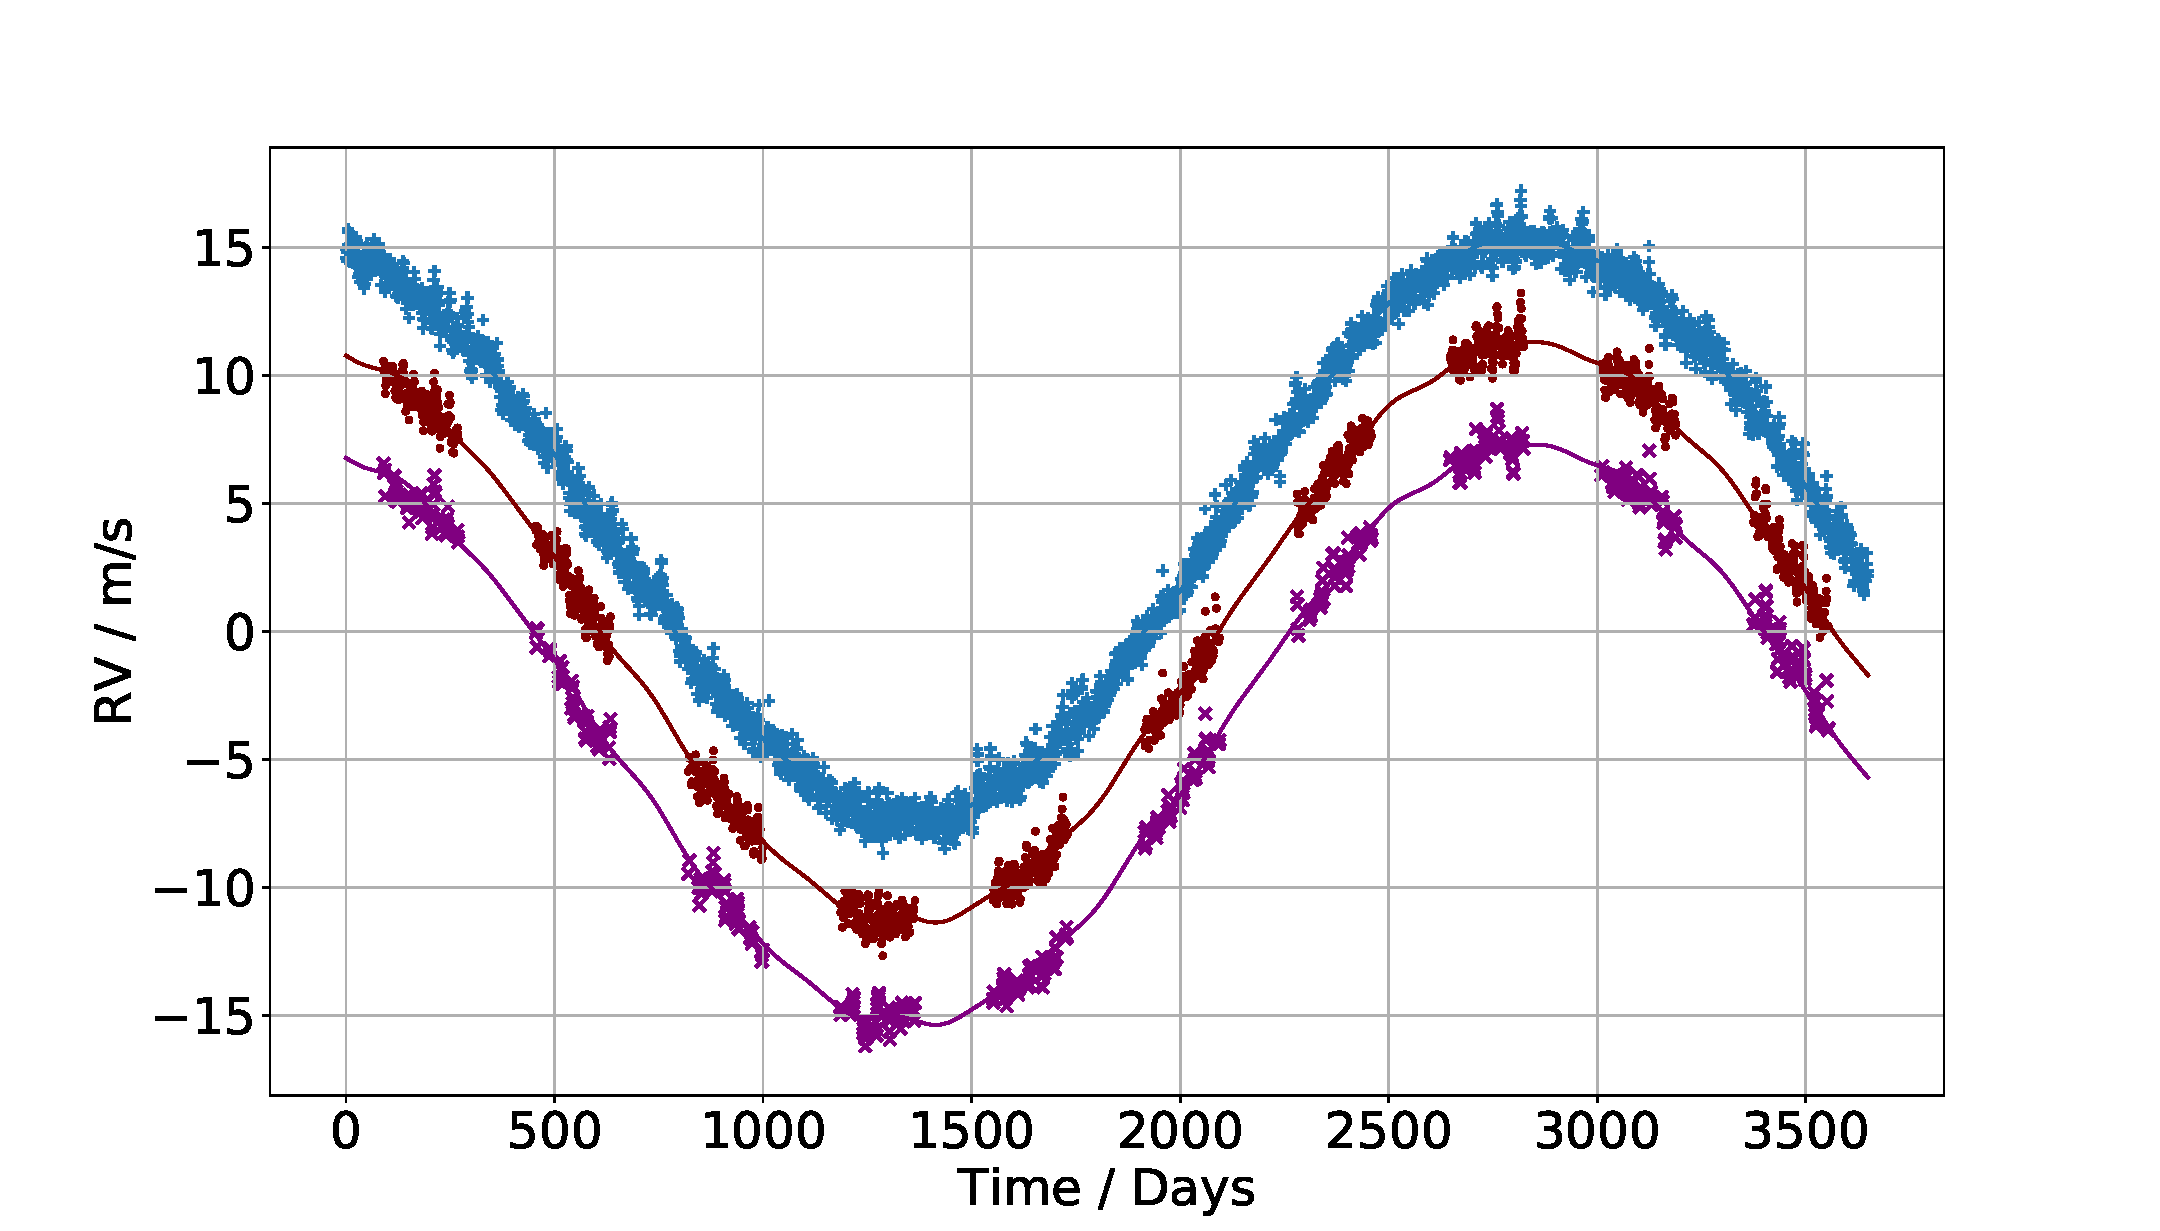
\includegraphics[width=\textwidth]{figures/rv_full.pdf}
\end{frame}
\begin{frame}
  \frametitle{Example: Exoplanets}
  \begin{itemize}
      \item Simple radial velocity model
          \begin{equation}
              \nu(t;\theta) = \sum_{p=1}^N K_p \sin(\omega_p t + \phi_p)\nonumber
          \end{equation}
      \item Fit each model to data.
      \item Posteriors on model parameters $[(K_p,\omega_p,\phi_p),p=1\cdots N]$ quantify knowledge of system characteristics.
      \item Evidences of models determine relative likelihood of number of planets in system
      \item \href{https://arxiv.org/abs/1806.00518}{arXiv:1806.00518}
  \end{itemize}
\end{frame}

\begin{frame}
  \frametitle{Example: function $\PR(k)$ reconstruction}


  \resizebox{\textwidth} {!} {%
    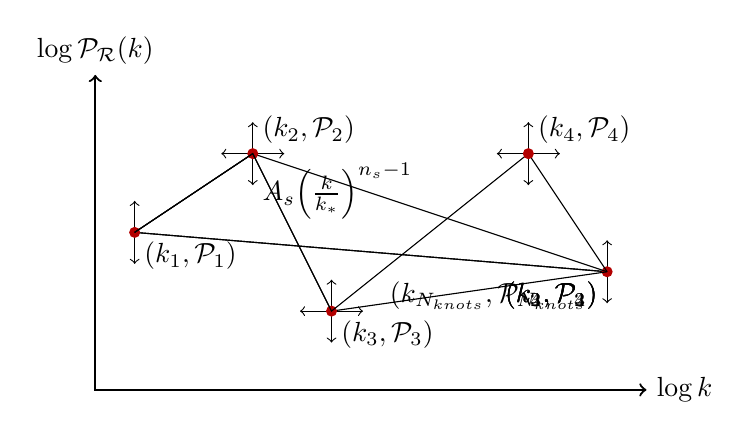
\begin{tikzpicture}
    % width of axes
      \def\xwidth{7}
      \def\ywidth{4}
    % min coordinate
      \def\xmn{0.5}
      \def\ymn{2}
    % start coordinate
      \def\xstart{2}
      \def\ystart{3}
    % middle coordinate
      \def\xmid{3}
      \def\ymid{1}
    % end coordinate
      \def\xend{5.5}
      \def\yend{3}
    % max coordinate
      \def\xmx{6.5}
      \def\ymx{1.5}

    % length of crosses
      \def\croslen{0.4}


    % Draw axes
      \draw [<->,thick] (0,\ywidth) node (yaxis) [above] {$\log\PR(k)$}
      |- (\xwidth,0) node (xaxis) [right] {$\log k$};
    % Draw limits
      %\draw [-,dashed] (\xmn,0) node[below] {$\log_{10}k_1$} -- (\xmn,\ywidth) ;
      %\draw [-,dashed] (\xmx,0) node[below] {$\log_{10}k_N$} -- (\xmx,\ywidth) ;

      \draw<1> (\xmn,\ymn) -- (\xmx,\ymx);
      \draw<1> (\xstart,\ystart) node[below right] {$A_s {\left(\frac{k}{k_*}\right)}^{n_s-1}$};

    % Draw the line joining start and end

      \coordinate (mn) at (\xmn,\ymn);
      \coordinate (start) at (\xstart,\ystart);
      \coordinate (mid) at (\xmid,\ymid);
      \coordinate (end) at (\xend,\yend);
      \coordinate (mx) at (\xmx,\ymx);
      \draw<2> (mn) -- (mx);
      \draw<2-> (mn) node[below right]    {$(k_1,\Pknotj{1})$};
      \draw<2> (mx) node[below left]     {$(k_{2},\Pknotj{{2}})$};
      \onslide<2->{\movablevert{mn}};
      \onslide<2->{\movablevert{mx}};

      \draw<3> (mn) -- (start) -- (mx);
      \onslide<3->{\movablecross{start}};
      \draw<3-> (start) node[above right] {$(k_2,\Pknotj{2})$};
      \draw<3> (mx) node[below left]     {$(k_{3},\Pknotj{{3}})$};
 
      \draw<4> (mn) -- (start) -- (mid) -- (mx);
      \onslide<4->{\movablecross{mid}};
      \draw<4-> (mid) node[below right] {$(k_3,\Pknotj{3})$};
      \draw<4> (mx) node[below left]     {$(k_{4},\Pknotj{{4}})$};

      \draw<5-> (mn) -- (start) -- (mid) -- (end) -- (mx);
      \onslide<5->{\movablecross{end}};
      \draw<5-> (end) node[above right] {$(k_4,\Pknotj{4})$};
      \draw<5-> (mx) node[below left]     {$(k_{\Nknots},\Pknotj{{\Nknots}})$};


      %\draw<2-> (\xmn,\ymn) coordinate (mn) -- (\xstart,\ystart) coordinate (start) -- (\xmid,\ymid) coordinate (mid) --  (\xend,\yend) coordinate(end) -- (\xmx,\ymx) coordinate(mx);

    % Draw the point labels
      %\draw<2-> (mn) node[below right]    {$(k_1,\Pknotj{1})$};
      %\draw<2-> (start) node[above right] {$(k_2,\Pknotj{2})$};
      %\draw<2-> (mid) node[below right]   {$(k_3,\Pknotj{3})$};
      %\draw<2-> (end) node[above right]   {$(k_4,\Pknotj{4})$};
      %\draw<2-> (mx) node[below left]     {$(k_{\Nknots},\Pknotj{{\Nknots}})$};

    % Draw a dashed line indicating the coordinate names
      %\draw[dashed] (yaxis |- start) node[left] {$y_{1}$}
      %-| (xaxis -| start) node[below] {$x_1$};
      %\draw[dashed] (yaxis |- mid) node[left] {$y_{2}$}
      %-| (xaxis -| mid) node[below] {$x_2$};
      %\draw[dashed] (yaxis |- end) node[left] {$y_{N}$}
      %-| (xaxis -| end) node[below] {$x_N$};
      %\draw  (xaxis -| start) node[below] {$\log_{10}k_2$};
      %\draw  (xaxis -| mid) node[below] {$\log_{10}k_3$};
      %\draw  (xaxis -| end) node[below] {$\log_{10}k_4$};

      % Draw the crosses
      %\onslide<2->{\movablevert{mn}
      %\movablecross{start}
      %\movablecross{mid}
      %\movablecross{end}
      %\movablevert{mx}
    %};

    % put some ellipses in between the start and end point

    \end{tikzpicture}

  }

\end{frame}
%
%
%
\begin{frame}
  \frametitle<1>{no tilt}
  \frametitle<2>{tilted}
  \frametitle<3>{1 internal knot}
  \frametitle<4>{2 internal knots}
  \frametitle<5>{3 internal knots}
  \frametitle<6>{4 internal knots}
  \frametitle<7>{5 internal knots}
  \frametitle<8>{6 internal knots}
  \frametitle<9>{7 internal knots}
  \frametitle<10>{Bayes Factors}
  \frametitle<11>{Marginalised plot}
  \framesubtitle{Primordial power spectrum $\PR(k)$ reconstruction}


  \begin{center}
    \includegraphics<1>[width=0.6\textwidth]{figures/pps_1}
    \includegraphics<2>[width=0.6\textwidth]{figures/pps_2}
    \includegraphics<3>[width=0.6\textwidth]{figures/pps_3}
    \includegraphics<4>[width=0.6\textwidth]{figures/pps_4}
    \includegraphics<5>[width=0.6\textwidth]{figures/pps_5}
    \includegraphics<6>[width=0.6\textwidth]{figures/pps_6}
    \includegraphics<7>[width=0.6\textwidth]{figures/pps_7}
    \includegraphics<8>[width=0.6\textwidth]{figures/pps_8}
    \includegraphics<9>[width=0.6\textwidth]{figures/pps_9}
    \includegraphics<10>[width=0.49\textwidth]{figures/pps_dkl}
    \includegraphics<10>[width=0.49\textwidth]{figures/pps_evidence}
    \includegraphics<11>[width=0.6\textwidth]{figures/pps.pdf}

  \end{center}
\end{frame}

\end{document}
